\documentclass{ltjsarticle} %lualatex cs_jikken.texで作成 
\usepackage{mdframed}
\usepackage{graphicx}
\usepackage{float}
\usepackage{array}
\usepackage{tikz}
\usetikzlibrary{automata, positioning, arrows}
\begin{document}

\thispagestyle{empty}
\begin{flushright}
{\large 実験実施日 2024年10月3日{\hspace{5cm}}} 
\end{flushright}

\vspace*{\fill}
\centering
{\Huge\bf コンピュータ科学実験b}
\vspace*{1cm}

{\huge\bf ハードウェア}
\vspace*{\fill}

\vspace*{\fill}

\vspace*{\fill}

\begin{flushright}
{\large 学生番号: 102210017} \\ % 5cmの空白を作り、アンダーラインを引く
{\large 氏名: 安藤駿} \\
{\large 共同実験者: 鬼頭海吏}
\end{flushright}

\clearpage

\addtocounter{page}{-1}
\raggedright
\setlength{\parindent}{1em}
\section{はじめに}
本実験では, コンピュータ科学の基礎について, 講義・演習などで得た知識を実験を通して検証・体得
し, コンピュータ科学の基礎となるシステムの構築に関して, 実際に計算機ハードウェアおよびソフトウェ
アのシステムを構築することにより, その構成法を体得することを目的とする.

\section{課題1 PC/AT互換機の部品知識とPCの組み⽴て}

\subsection{目的・概要}
IBM-PC/AT互換パソコン(PC)の組み⽴てを通してパソコンの部品, 標準インタフェース, マザーボード
のBIOSなどについての知識を獲得する. 

\subsection{IBM-PC/AT互換機に使われる部品}

\subsubsection{マザーボード}
マザーボードは, PC/AT互換パソコンの最も基本的な構成要素を搭載する重要な回路基板である.
本実験で使用する製品は,  Supermicro社のX11SCZ-Qである. 図\ref{fig:mother1}に示す.

\begin{figure}[H] % 画像を挿入する環境を開始
  \centering
  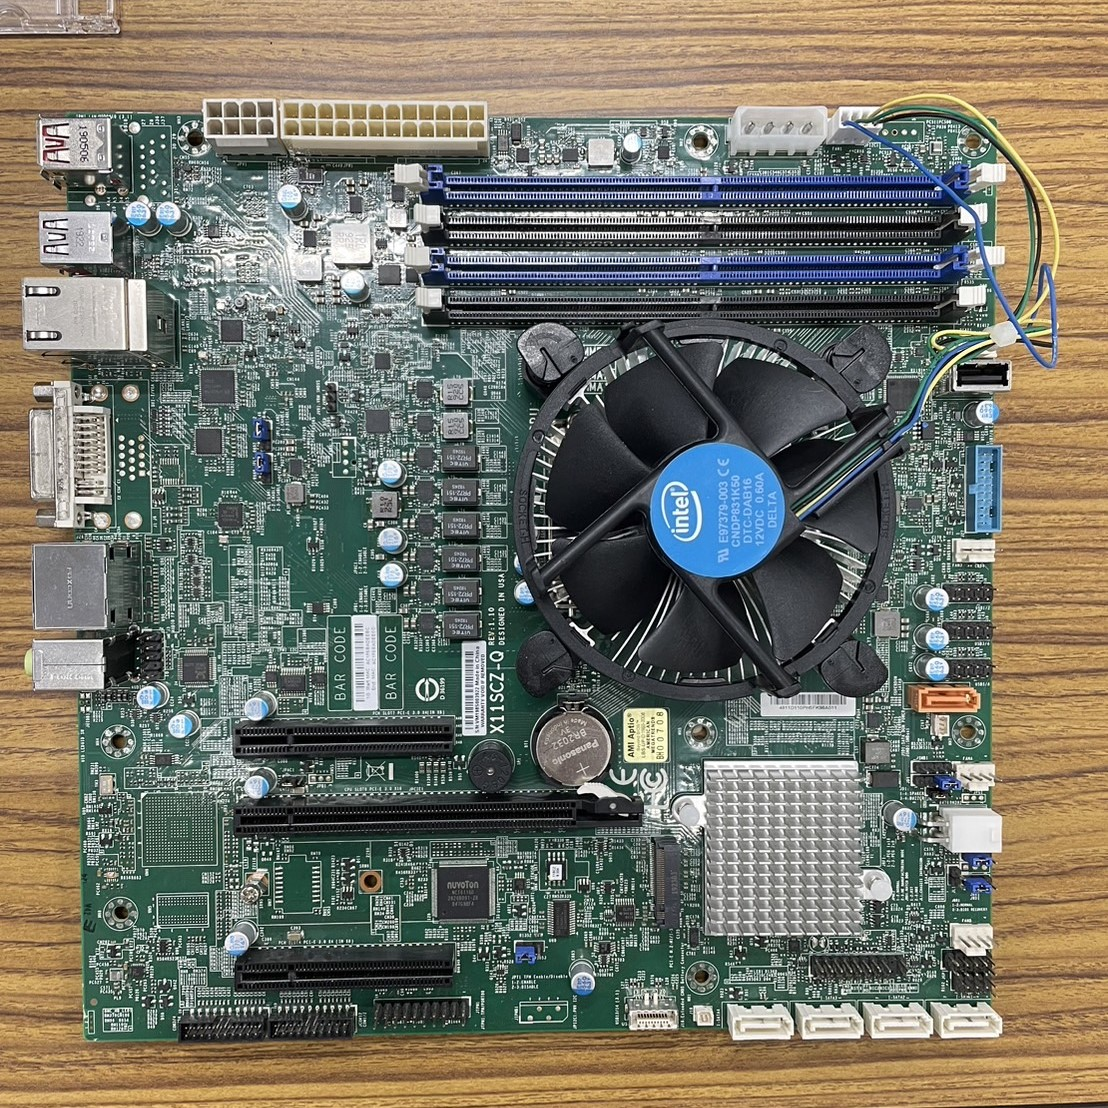
\includegraphics[width=0.5\textwidth]{mother1.jpg} % 画像を挿入、幅をページ幅に合わせる
  \caption{マザーボード} % キャプションを追加
  \label{fig:mother1} % ラベルを追加
\end{figure}

\subsubsection{ケース}
本実験ではタワー型ケースを使用した. 図\ref{fig:case1}に示す.
使用する製品は, THIRDWAVE社の715625-78900である. シリアル番号は, 16297038500439である. 

\begin{figure}[H] % 画像を挿入する環境を開始
  \centering
  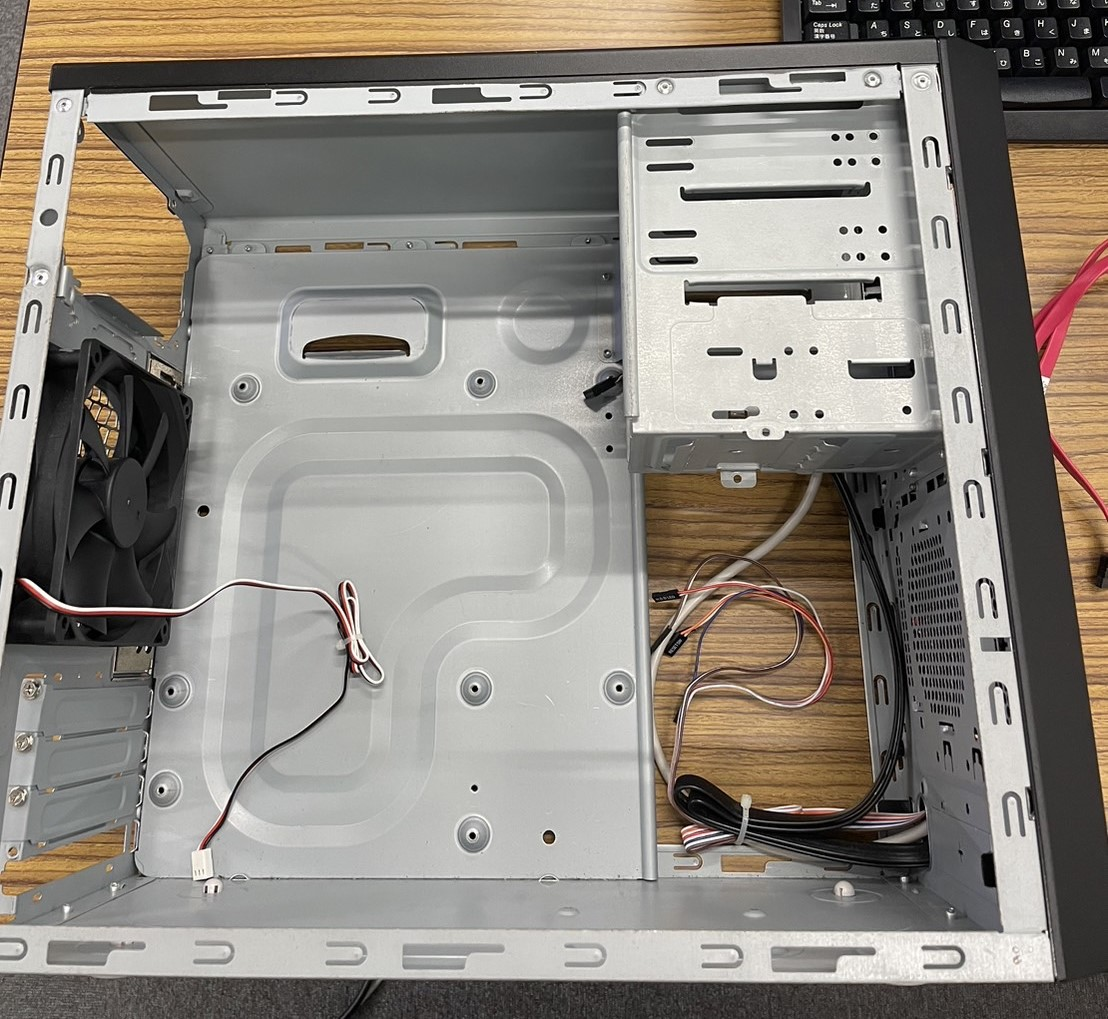
\includegraphics[width=0.5\textwidth]{case1.jpg} % 画像を挿入、幅をページ幅に合わせる
  \caption{ケース} % キャプションを追加
  \label{fig:case1} % ラベルを追加
\end{figure}

\subsubsection{電源ユニット}
本実験で使用する製品は,  Acbel社のPCA013である. シリアル番号は, PCA01319270015624Bである. 図\ref{fig:dengen3}に示す.

\begin{figure}[H] % 画像を挿入する環境を開始
  \centering
  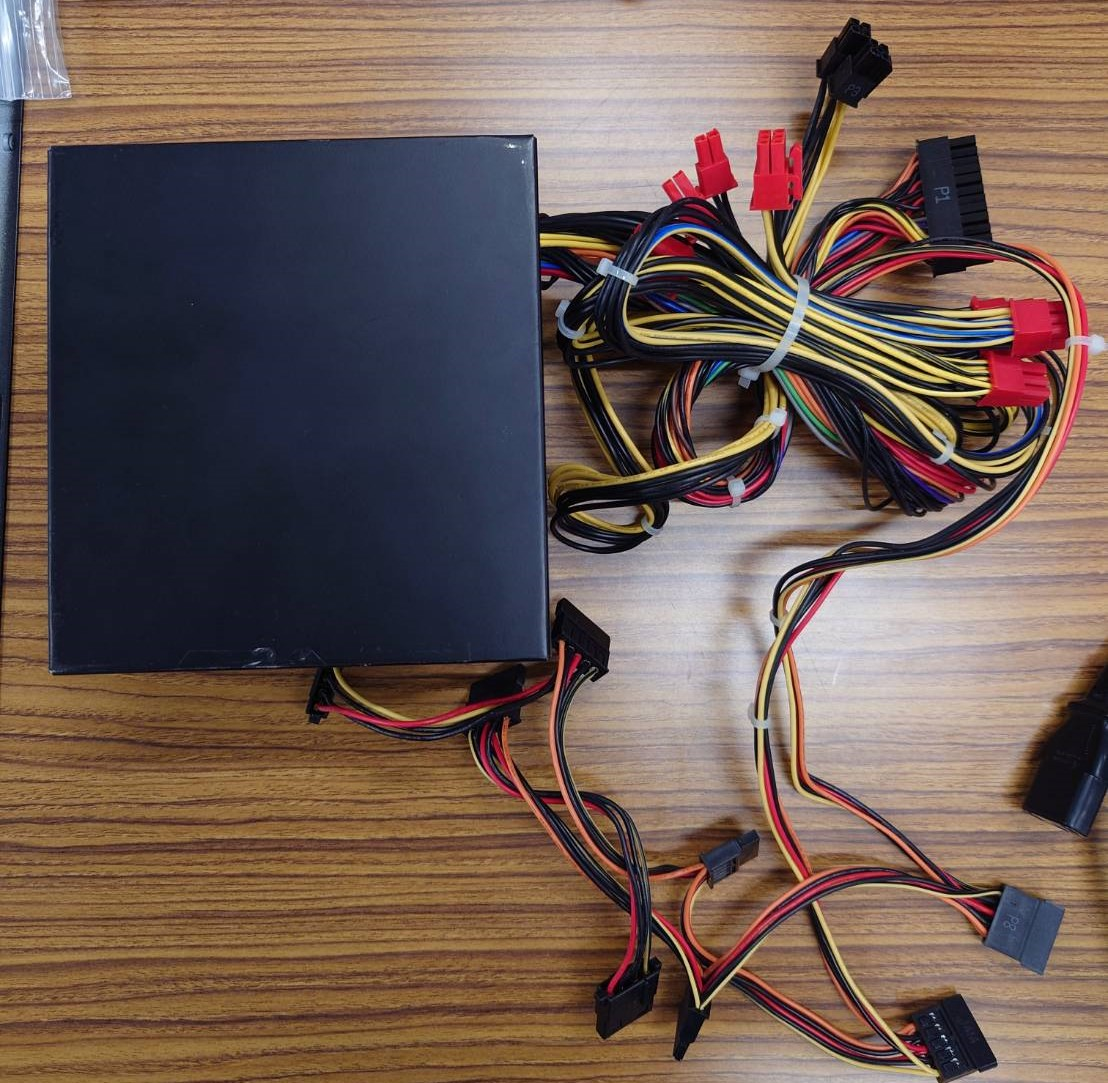
\includegraphics[width=0.5\textwidth]{dengen3.jpg} % 画像を挿入、幅をページ幅に合わせる
  \caption{電源ユニット} % キャプションを追加
  \label{fig:dengen3} % ラベルを追加
\end{figure}


\subsubsection{CPUとCPUクーラ}
CPU (Central Processing Unit)は, 中央処理装置もしくは中央演算処理装置と呼ばれ, 機における中⼼的な回路である.
本実験で使用するCPUは, Intel社のcore i5-8400である. 

CPUは動作時に熱を発⽣し, ⾼温になると能⼒の低下・熱暴⾛を起こす.
したがって, CPUを冷却するCPUクーラは重要な部品である.
本実験で使用するCPUクーラは, Intel E97379-003である. シリアル番号は, CNDP831K50である. 図\ref{fig:cpufan}に示す.

\begin{figure}[H] % 画像を挿入する環境を開始
  \centering
  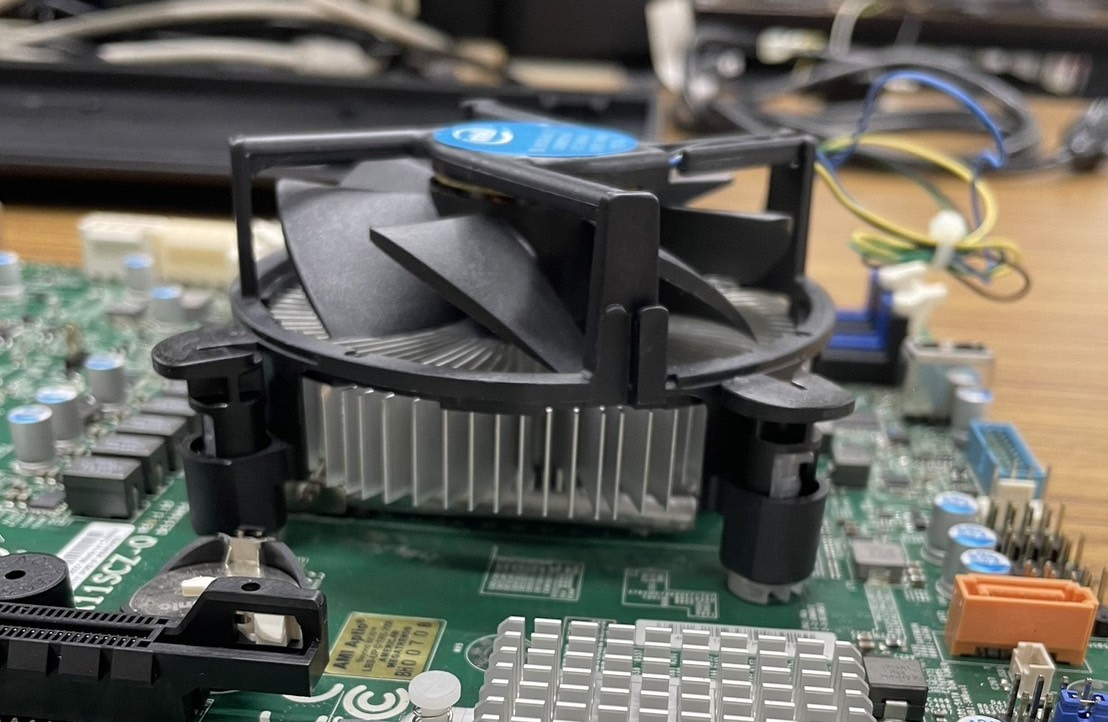
\includegraphics[width=0.5\textwidth]{cpufan.jpg} % 画像を挿入、幅をページ幅に合わせる
  \caption{CPU, CPUクーラ} % キャプションを追加
  \label{fig:cpufan} % ラベルを追加
\end{figure}


\subsubsection{メインメモリ(DRAM)}
Dynamic Random Access Memoryとも呼ばれ, 計算機のメインメモリとして使⽤される.
本実験で使用する製品は,  hma851u6cjr6n-vkである. シリアル番号は, 43351F30と43351EF8である. 図\ref{fig:dram2}に示す. 

\begin{figure}[H] % 画像を挿入する環境を開始
  \centering
  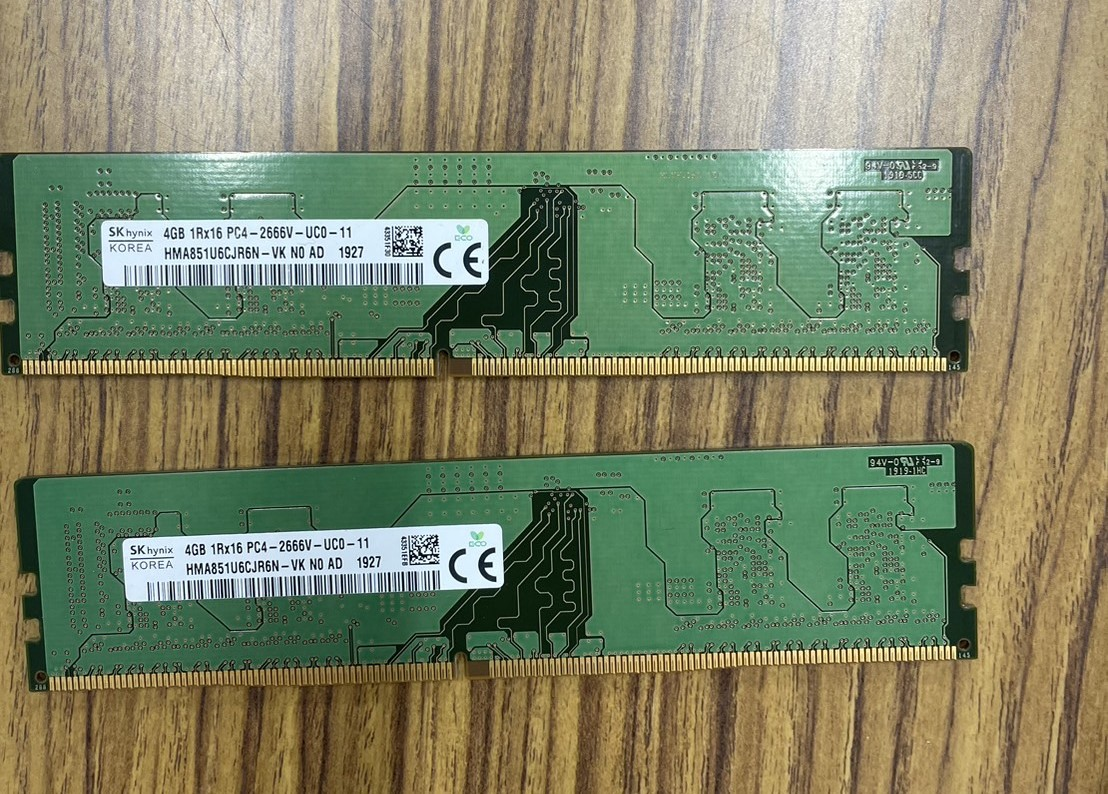
\includegraphics[width=0.5\textwidth]{dram2.jpg} % 画像を挿入、幅をページ幅に合わせる
  \caption{DRAM} % キャプションを追加
  \label{fig:dram2} % ラベルを追加
\end{figure}


\subsubsection{拡張カードスロット}
本実験で使用する拡張カードスロットは, パラレルポートおよびシリアルポートを追加する. 
本実験で使用する製品は, ART3 2SSP 1803である. 図\ref{fig:port}に示す.

\begin{figure}[H] % 画像を挿入する環境を開始
  \centering
  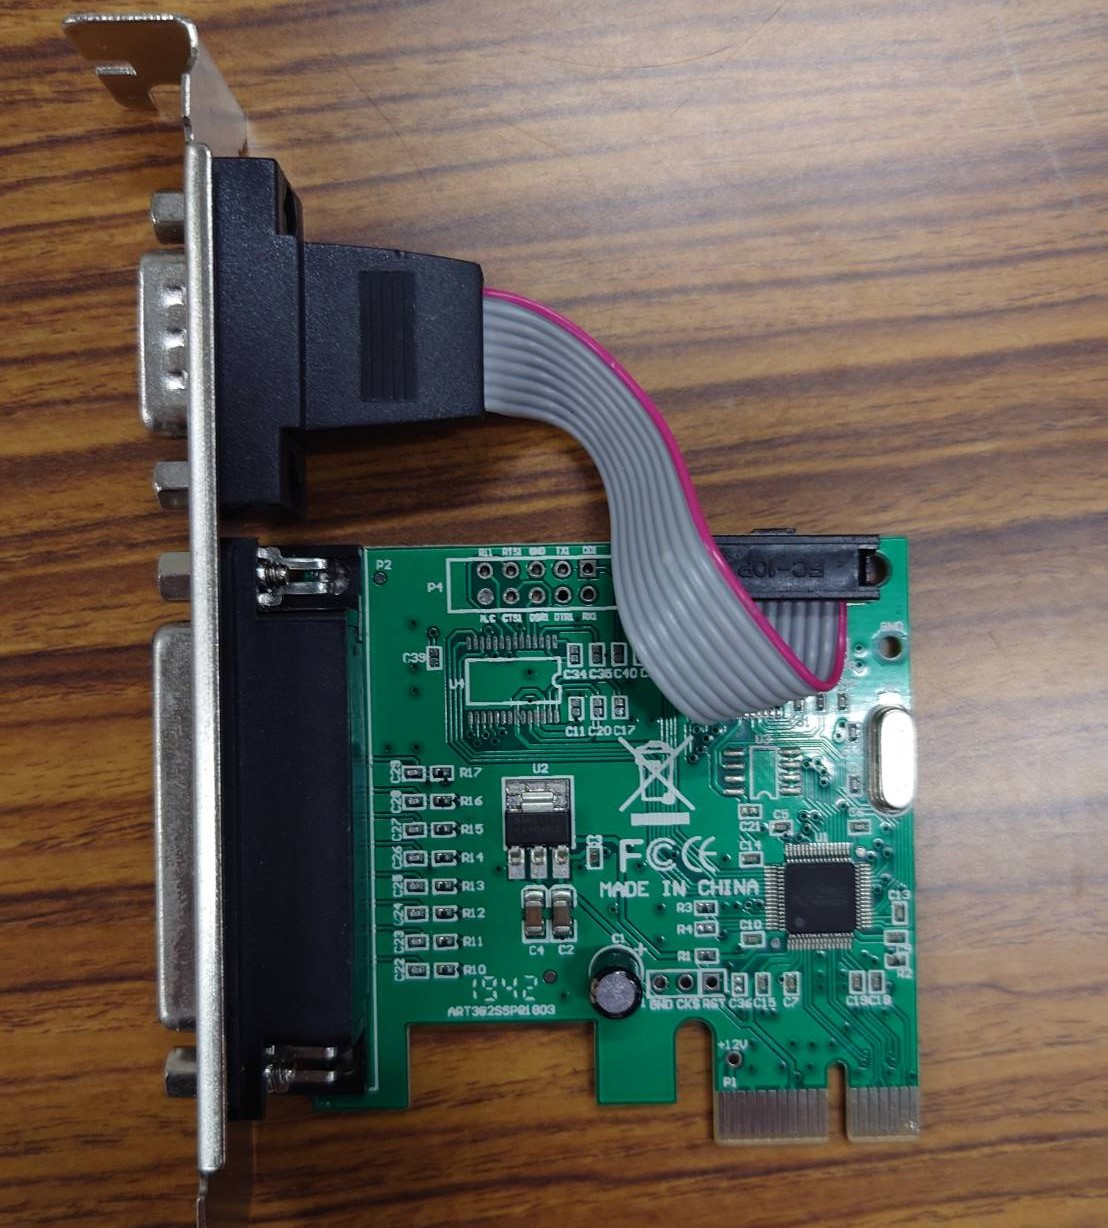
\includegraphics[width=0.5\textwidth]{port.jpg} % 画像を挿入、幅をページ幅に合わせる
  \caption{拡張カードスロット} % キャプションを追加
  \label{fig:port} % ラベルを追加
\end{figure}


\subsubsection{ソリッドステートドライブ (SSD)}
ソリッドステートドライブは, 記憶装置として半導体メモリを使⽤したデバイスである.
本実験で使用する製品は, Western Digital社のWDS250G2B0Aである. シリアル番号は, 00SM50である. 図\ref{fig:ssd1}に示す.

\begin{figure}[H] % 画像を挿入する環境を開始
  \centering
  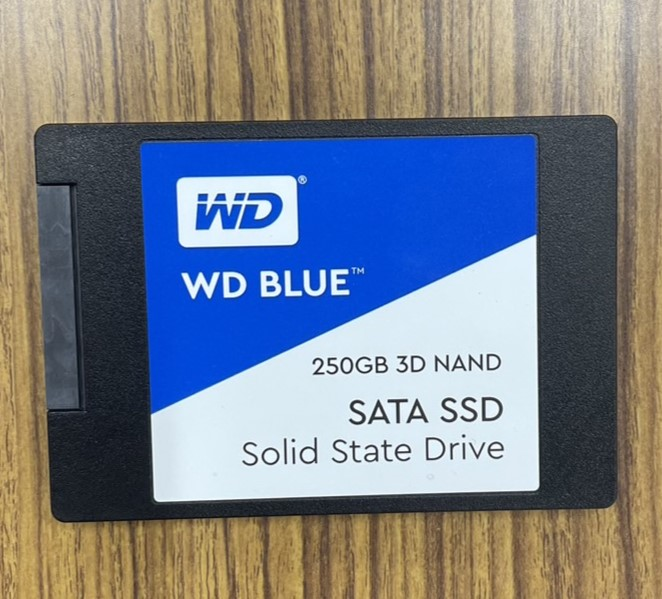
\includegraphics[width=0.5\textwidth]{ssd1.jpg} % 画像を挿入、幅をページ幅に合わせる
  \caption{SSD} % キャプションを追加
  \label{fig:ssd1} % ラベルを追加
\end{figure}


\subsubsection{光学ドライブ}
CD-ROMやDVD-ROMやBlu-ray Discを読み書き可能なドライブを総称して光学ドライブと呼ぶ.
本実験で使用する製品は,  H.L Data Storage社のDH18NS61である. シリアル番号は, 906HAZX053733である. 図\ref{fig:cd1}に示す. 

\begin{figure}[H] % 画像を挿入する環境を開始
  \centering
  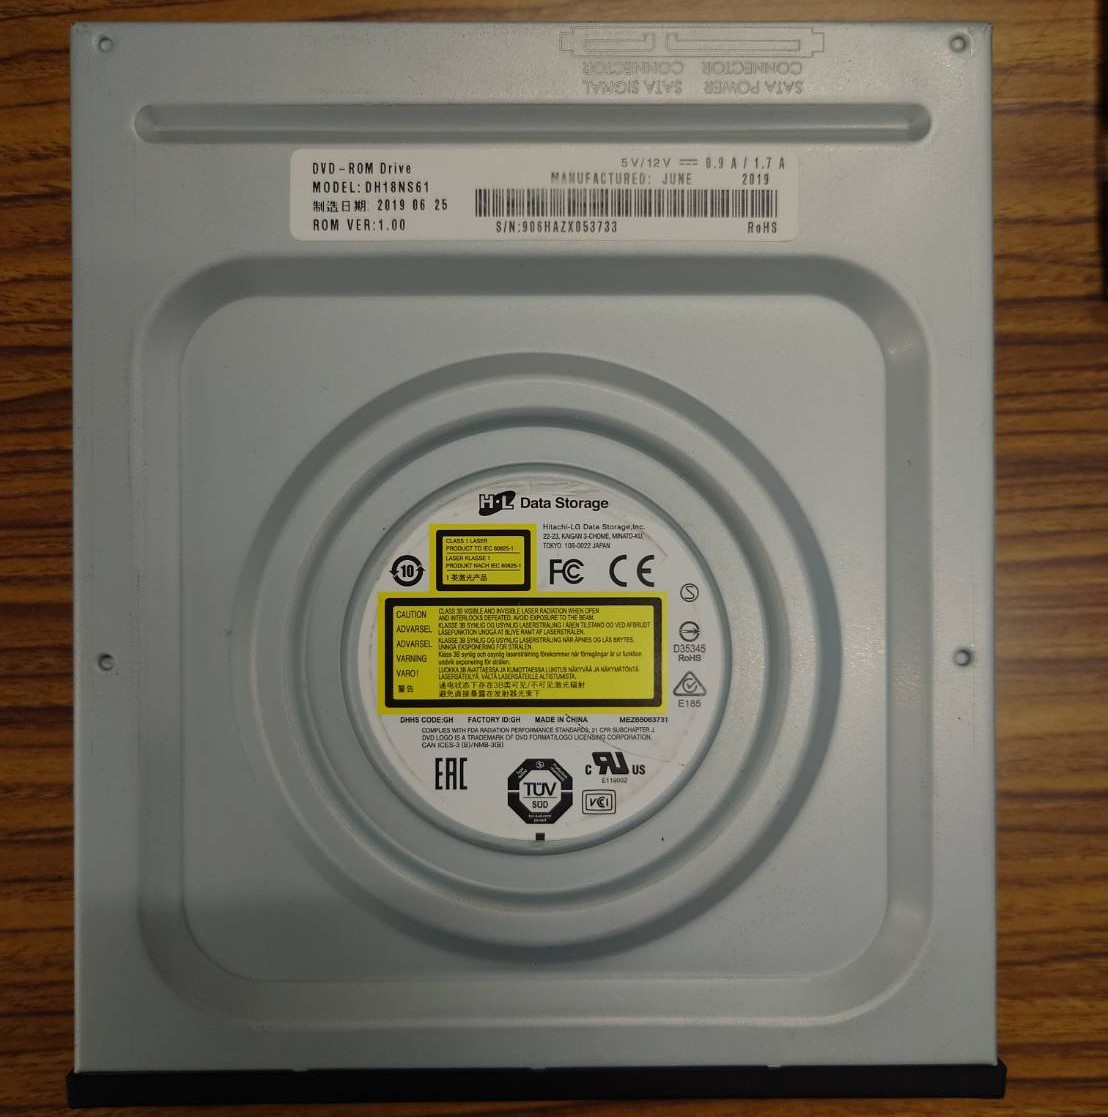
\includegraphics[width=0.5\textwidth]{cd1.jpg} % 画像を挿入、幅をページ幅に合わせる
  \caption{光学ドライブ} % キャプションを追加
  \label{fig:cd1} % ラベルを追加
\end{figure}


\subsubsection{キーボード}
本実験で使用する製品の型番は, FKD46AK297である. シリアル番号は, M1907001286である. 図\ref{fig:keyboard}に示す.

\begin{figure}[H] % 画像を挿入する環境を開始
  \centering
  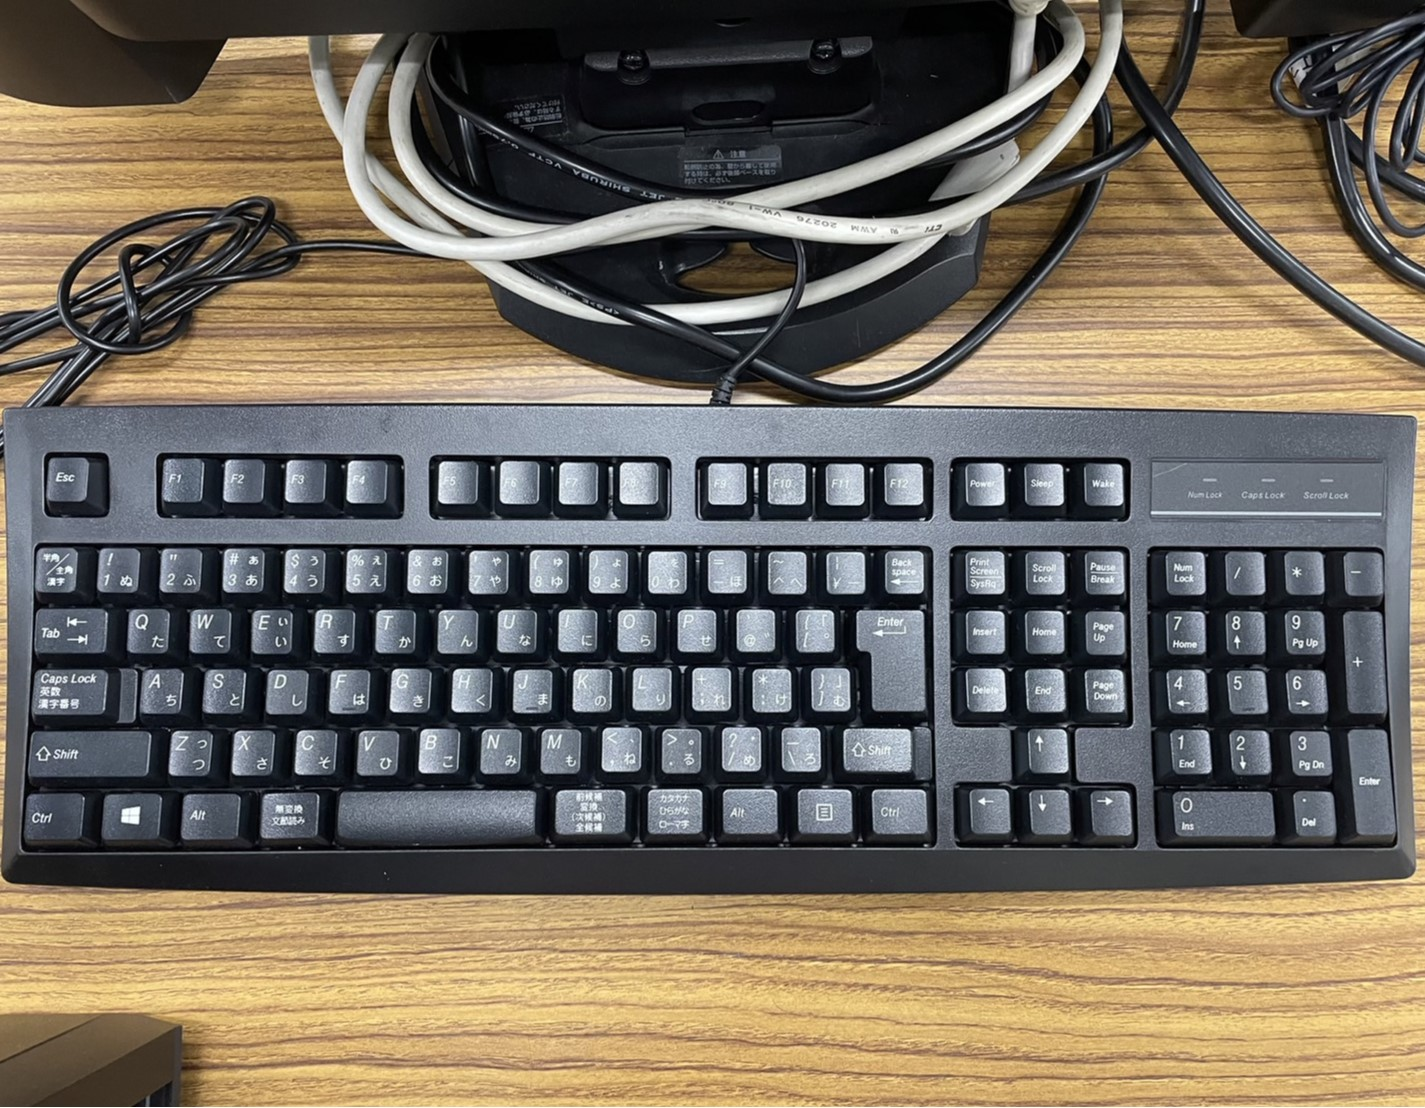
\includegraphics[width=0.5\textwidth]{keyboard.jpg} % 画像を挿入、幅をページ幅に合わせる
  \caption{キーボード} % キャプションを追加
  \label{fig:keyboard} % ラベルを追加
\end{figure}


\subsubsection{マウス}
本実験で使用する製品は, Microsoft社の1113である. 図\ref{fig:mouse1}に示す.

\begin{figure}[H] % 画像を挿入する環境を開始
  \centering
  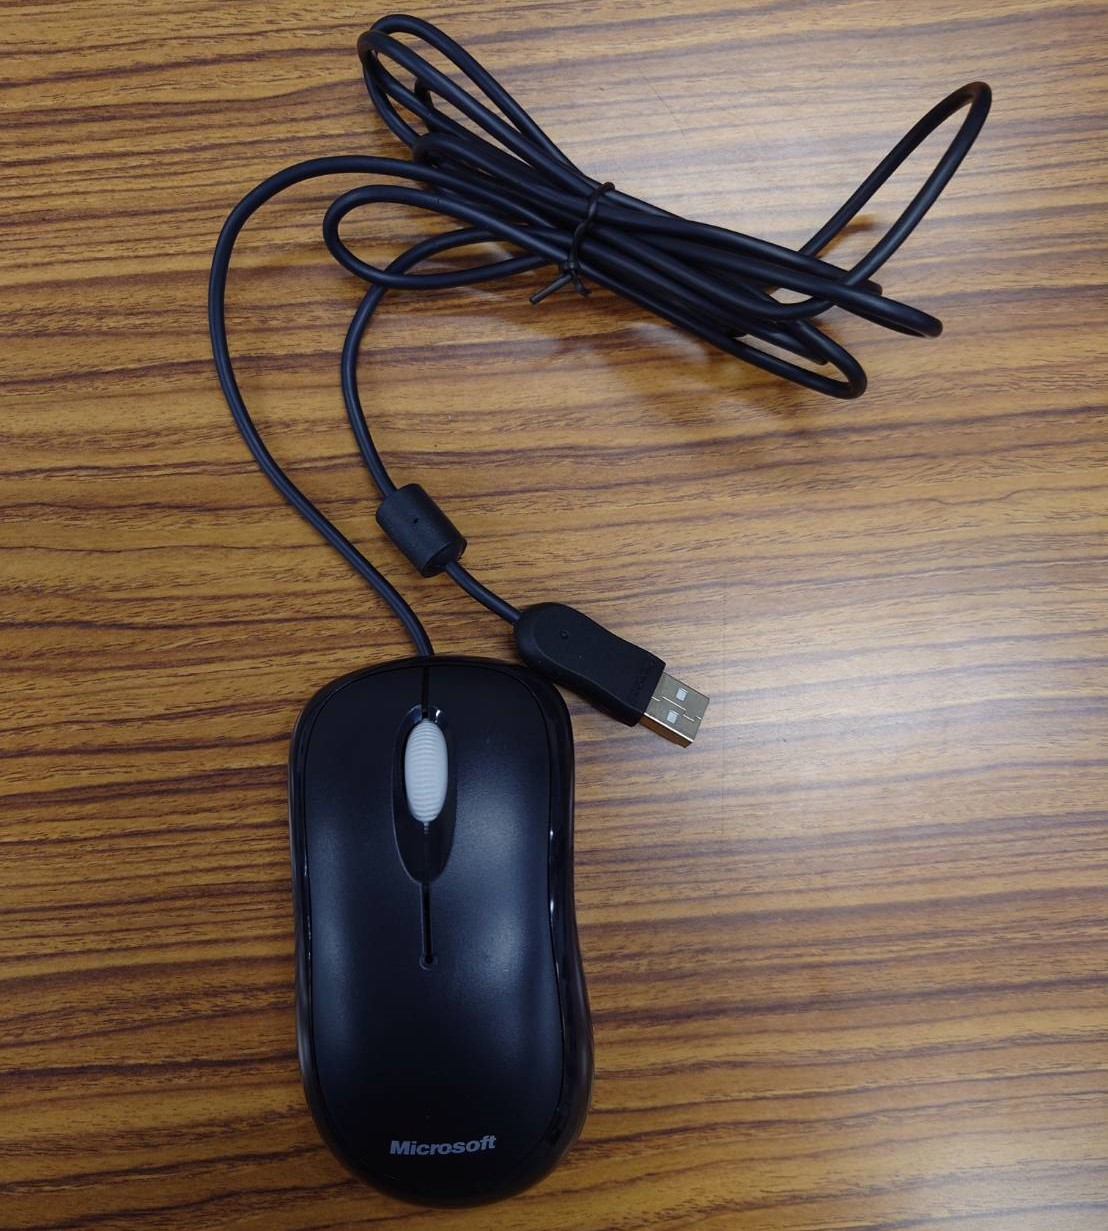
\includegraphics[width=0.5\textwidth]{mouse1.jpg} % 画像を挿入、幅をページ幅に合わせる
  \caption{マウス} % キャプションを追加
  \label{fig:mouse1} % ラベルを追加
\end{figure}


\subsubsection{モニタ}
本実験で使用する製品は,  三菱電機社のRDT232WXである. シリアル番号は, 11230693AJである. 図\ref{fig:monita}に示す.

\begin{figure}[H] % 画像を挿入する環境を開始
  \centering
  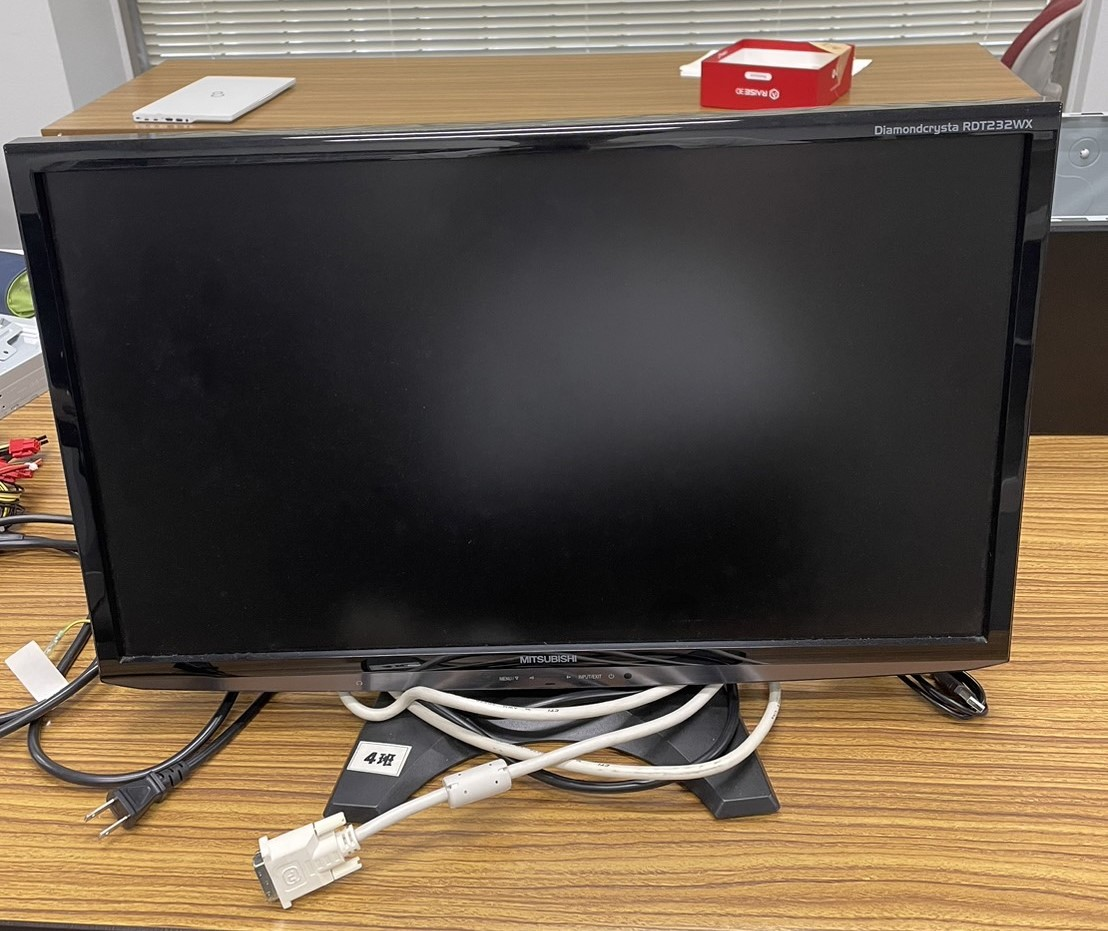
\includegraphics[width=0.5\textwidth]{monita.jpg} % 画像を挿入、幅をページ幅に合わせる
  \caption{モニタ} % キャプションを追加
  \label{fig:monita} % ラベルを追加
\end{figure}


\subsubsection{ミリネジ}
光学ドライブ, SSD用に使った. 図\ref{fig:neji1}に示す. 

\begin{figure}[H] % 画像を挿入する環境を開始
  \centering
  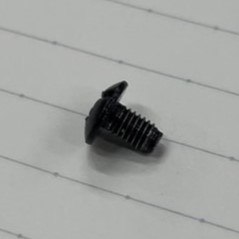
\includegraphics[width=0.5\textwidth]{neji1.jpg} % 画像を挿入、幅をページ幅に合わせる
  \caption{ミリネジ} % キャプションを追加
  \label{fig:neji1} % ラベルを追加
\end{figure}


\subsubsection{インチネジ}
ケース, 電源, マザーボード⽤に使った. 図\ref{fig:neji2}に示す.

\begin{figure}[H] % 画像を挿入する環境を開始
  \centering
  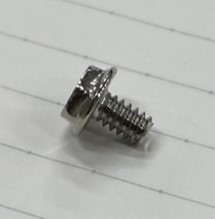
\includegraphics[width=0.5\textwidth]{neji2.jpg} % 画像を挿入、幅をページ幅に合わせる
  \caption{インチネジ} % キャプションを追加
  \label{fig:neji2} % ラベルを追加
\end{figure}


\subsubsection{SATAケーブル}
PCに取り付ける機器に対し, SATAケーブル使った. 図\ref{fig:SATA}に示す. 

\begin{figure}[H] % 画像を挿入する環境を開始
  \centering
  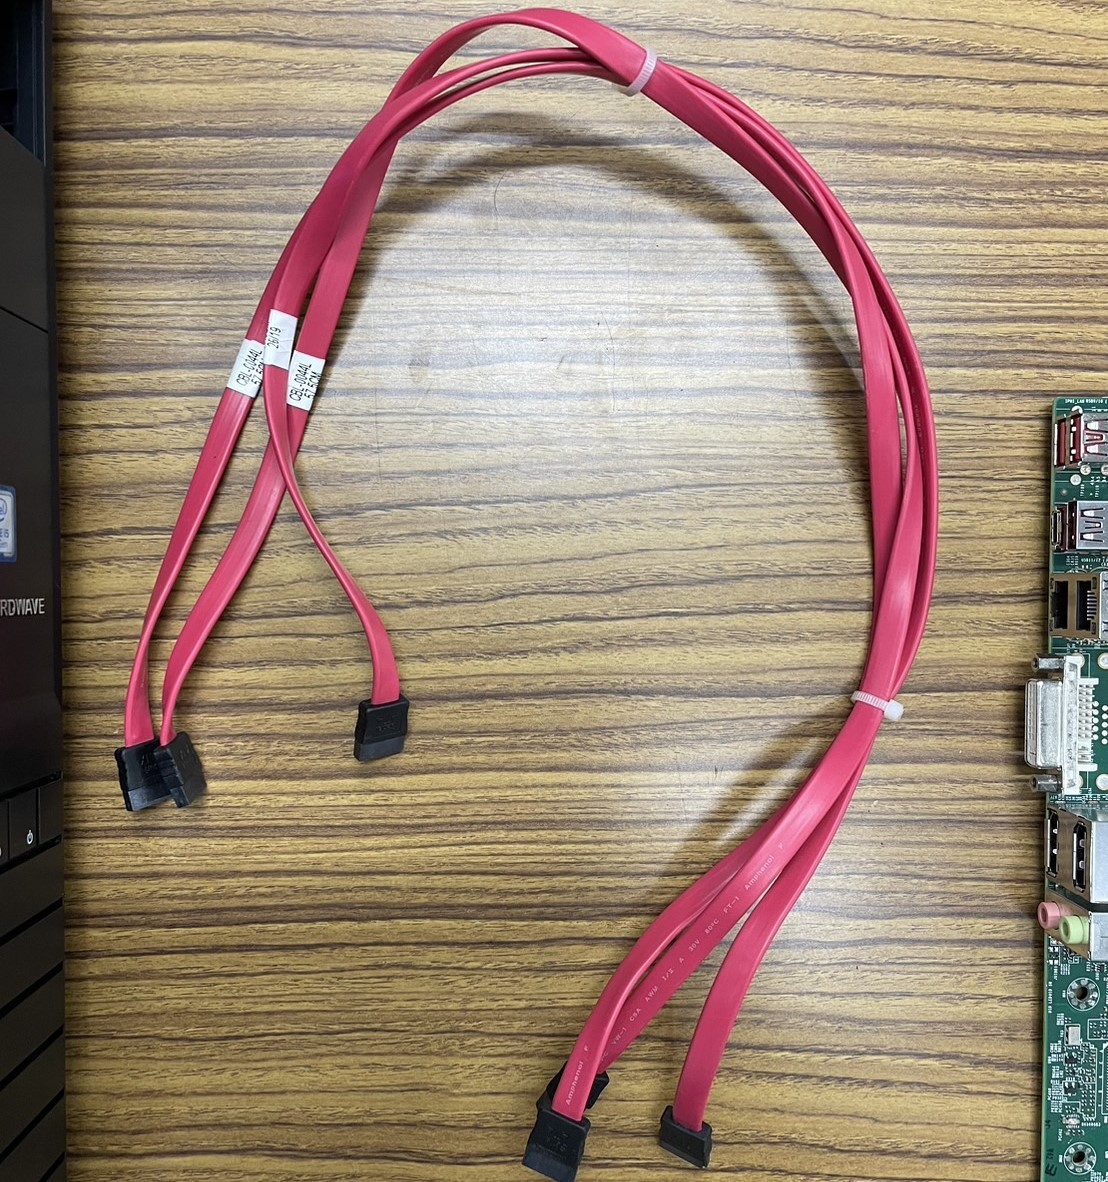
\includegraphics[width=0.5\textwidth]{SATA.jpg} % 画像を挿入、幅をページ幅に合わせる
  \caption{SATAケーブル} % キャプションを追加
  \label{fig:SATA} % ラベルを追加
\end{figure}


\subsection{実験方法}

\subsubsection{組⽴の準備}

プラスドライバを用意した.

\subsubsection{電源ユニットの取り付け}

ケースに電源ユニットを取り付け, インチネジで固定した. このときの状況を図\ref{fig:dengentoritsuke}に示す.

\begin{figure}[H] % 画像を挿入する環境を開始
  \centering
  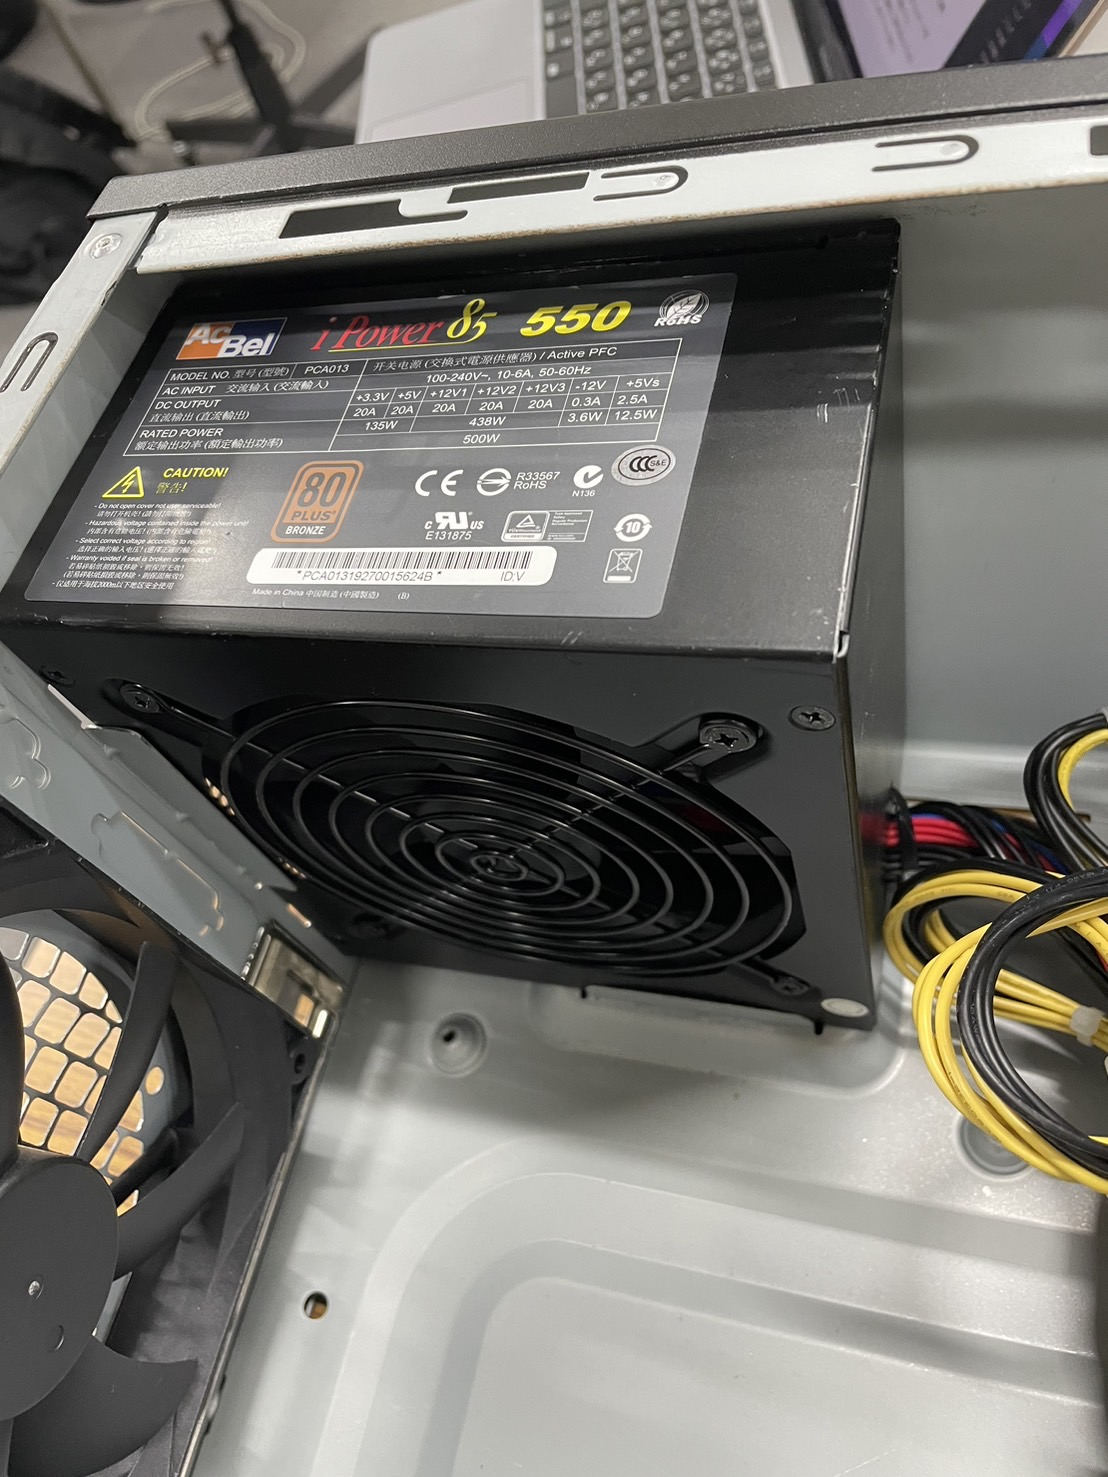
\includegraphics[width=0.5\textwidth]{dengentoritsuke.jpg} % 画像を挿入、幅をページ幅に合わせる
  \caption{ケースに取り付けた電源ユニット} % キャプションを追加
  \label{fig:dengentoritsuke} % ラベルを追加
\end{figure}

\subsubsection{メモリの取り付け}

2つのメモリモジュールを同じ色のソケットに差し込んだ. 十分に固定されていることを確認した.

\subsubsection{マザーボードと電源の取り付け}

マザーボードをケースに取り付け, インチネジで固定した. 
その後, 24ピンのTXメイン電源コネクタを図\ref{fig:chart1}に示すマザーボードの仕様書のJPW1に接続した. 
また, 補助電源として8ピンのATX12V電源ケーブルを図\ref{fig:chart1}のJPV1に接続した. 
この時の状況を図\ref{fig:mothertoritsuke}に示す.

\begin{figure}[H] % 画像を挿入する環境を開始
  \centering
  \begin{minipage}{0.45\textwidth} % 1つ目の画像の幅をページの45%に設定
    \centering
    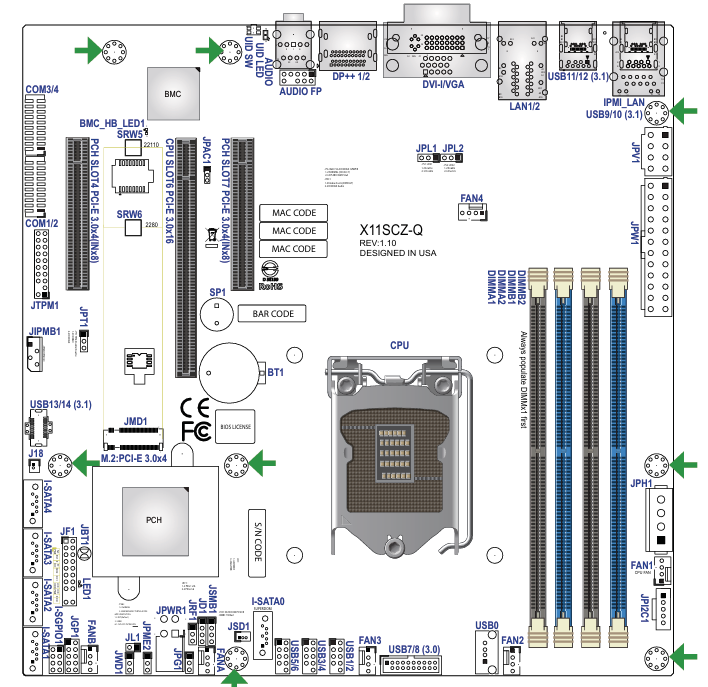
\includegraphics[width=\textwidth]{chart1.png} % 画像を挿入、幅をminipage幅に合わせる
    \caption{マザーボードの仕様書1} % キャプションを追加
    \label{fig:chart1} % ラベルを追加
  \end{minipage}
  \hfill % 画像の間にスペースを追加
  \begin{minipage}{0.45\textwidth} % 2つ目の画像の幅をページの45%に設定
    \centering
    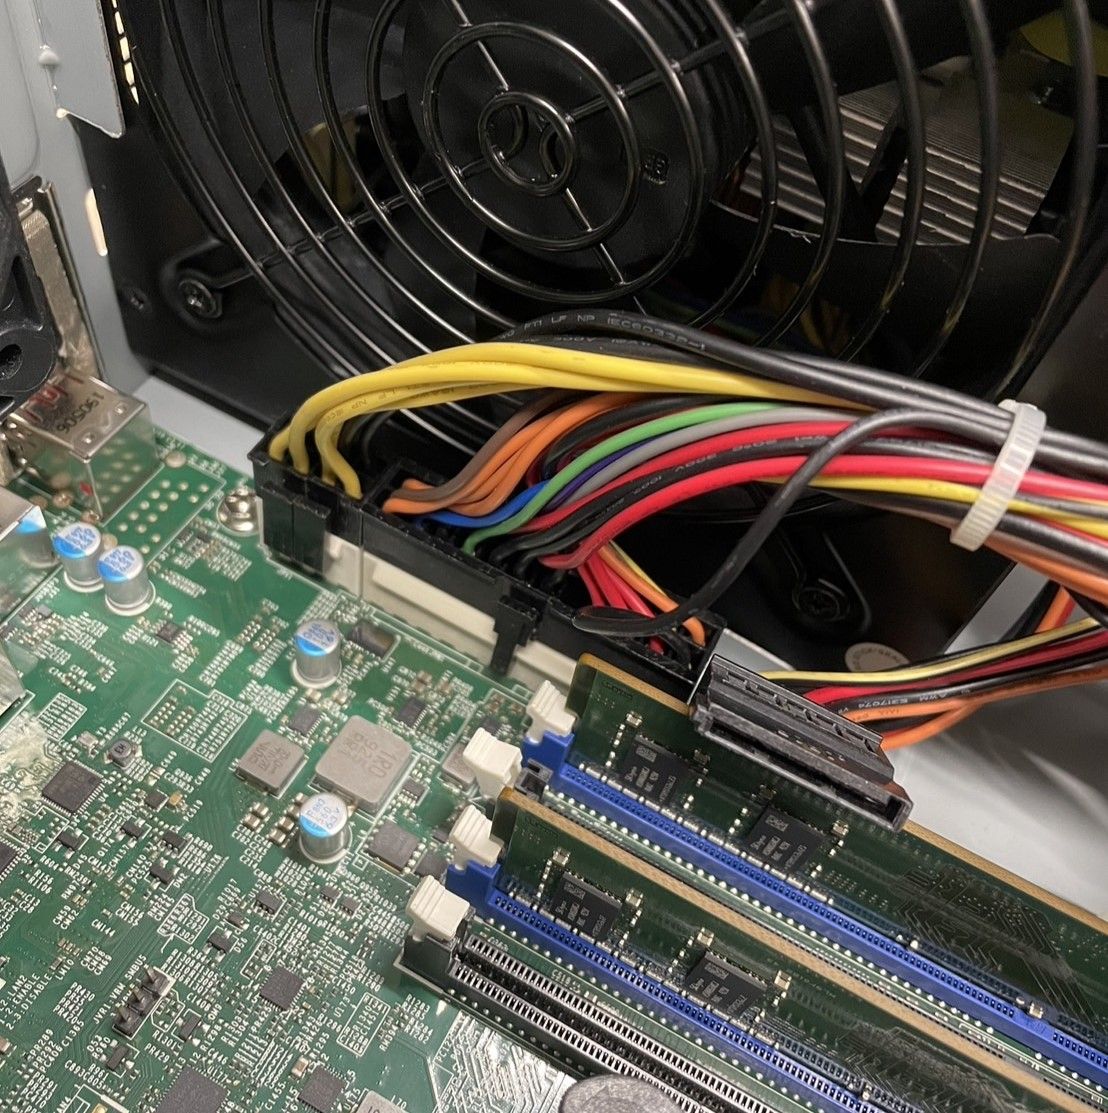
\includegraphics[width=\textwidth]{mothertoritsuke.jpg} % 2つ目の画像を挿入
    \caption{電源の取り付け} % キャプションを追加
    \label{fig:mothertoritsuke} % ラベルを追加
  \end{minipage}
\end{figure}


\subsubsection{ケースケーブル(アクセサリケーブル)の取り付け}

ケースのフロントパネルのスイッチとLED関連のケーブルを接続した.
具体的には, 図\ref{fig:chart2}のPOWER ButtonにPOWER SWを, 
Reset Buttonに RESET SWを,  HDD LEDに H.D.D LEDを, 
FP PWRLEDにPOWER LEDを接続した. ただし, 図\ref{fig:chart2}の左の列がプラスである.
このときの状況を図\ref{fig:casecable}に示す.
USBポートへつながるケーブルを図\ref{fig:chart1}のUSB7/8に接続し, 
排気ファンのケーブルを図\ref{fig:chart1}のFAN2に接続した. 

\begin{figure}[H] % 画像を挿入する環境を開始
  \centering
  \begin{minipage}{0.45\textwidth} % 1つ目の画像の幅をページの45%に設定
    \centering
    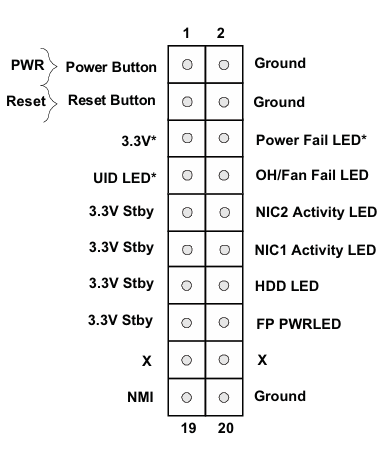
\includegraphics[width=\textwidth]{chart2.png} % 画像を挿入、幅をminipage幅に合わせる
    \caption{マザーボードの仕様書2} % キャプションを追加
    \label{fig:chart2} % ラベルを追加
  \end{minipage}
  \hfill % 画像の間にスペースを追加
  \begin{minipage}{0.45\textwidth} % 2つ目の画像の幅をページの45%に設定
    \centering
    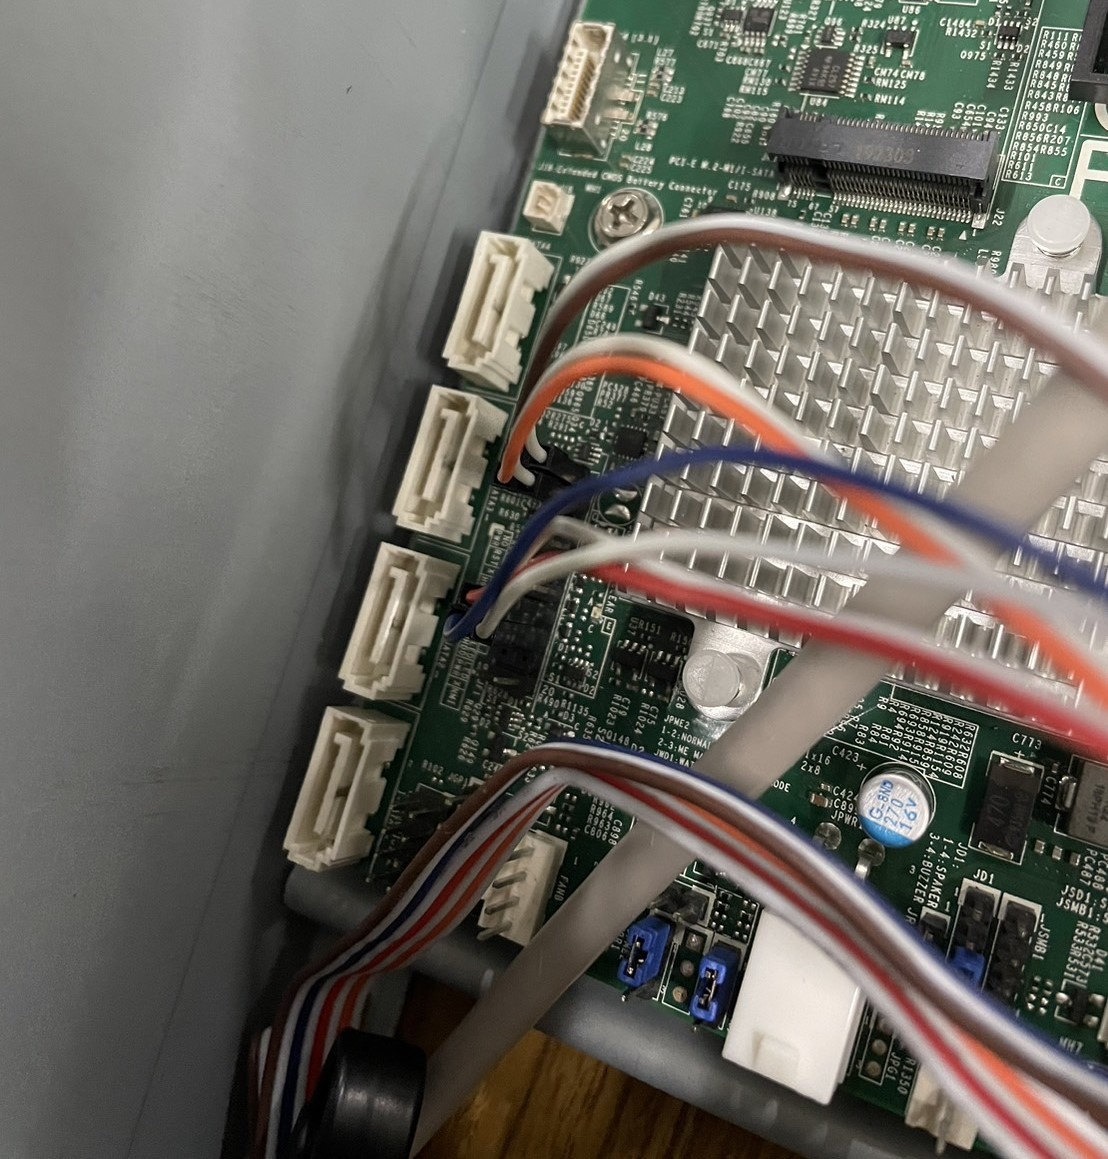
\includegraphics[width=\textwidth]{casecable.jpg} % 2つ目の画像を挿入
    \caption{スイッチとLED関連のケーブル} % キャプションを追加
    \label{fig:casecable} % ラベルを追加
  \end{minipage}
\end{figure}


\subsubsection{ドライブ類の装着}

SSDは2.5インチサイズなのでケースの3.5インチベイには直接取り付けできないため, 2.5インチサイ
ズに対応したマウンタにSSDを取り付け, マウンタをケースの3.5インチベイの下に取り付けた.
その後, インチネジでマウンタをケースに固定した.

光学ドライブを5インチベイに取り付け, ミリネジで固定した.

SSD と光学ドライブにSATAケーブルと電源ケーブルを接続した. SATAケーブルはマザーボードの図\ref{fig:chart1}の
SATA1, SATA2にも接続した.

\subsubsection{拡張カードの装着}

パラレルポートおよびシリアルポート増設カードを1枚装着し, インチネジで固定した.

\subsubsection{動作確認}
電源ケーブル, ディスプレイ, キーボード, マウスを接続し, ディスプレイの電源SWを投入した.
電源ユニットのスイッチを入れ, パソコンの電源を投⼊した.

ここで, DELETEキーを押し,  BIOS セットアップを起動した.
まずAdvanced画面から, CPUのモデル名を確認した. この時の状況を図\ref{fig:bios1}に示す.

次に, HDD, 光学ドライブがきちんと認識されているかどうかを確認した. 

\begin{figure}[H] % 画像を挿入する環境を開始
  \centering
  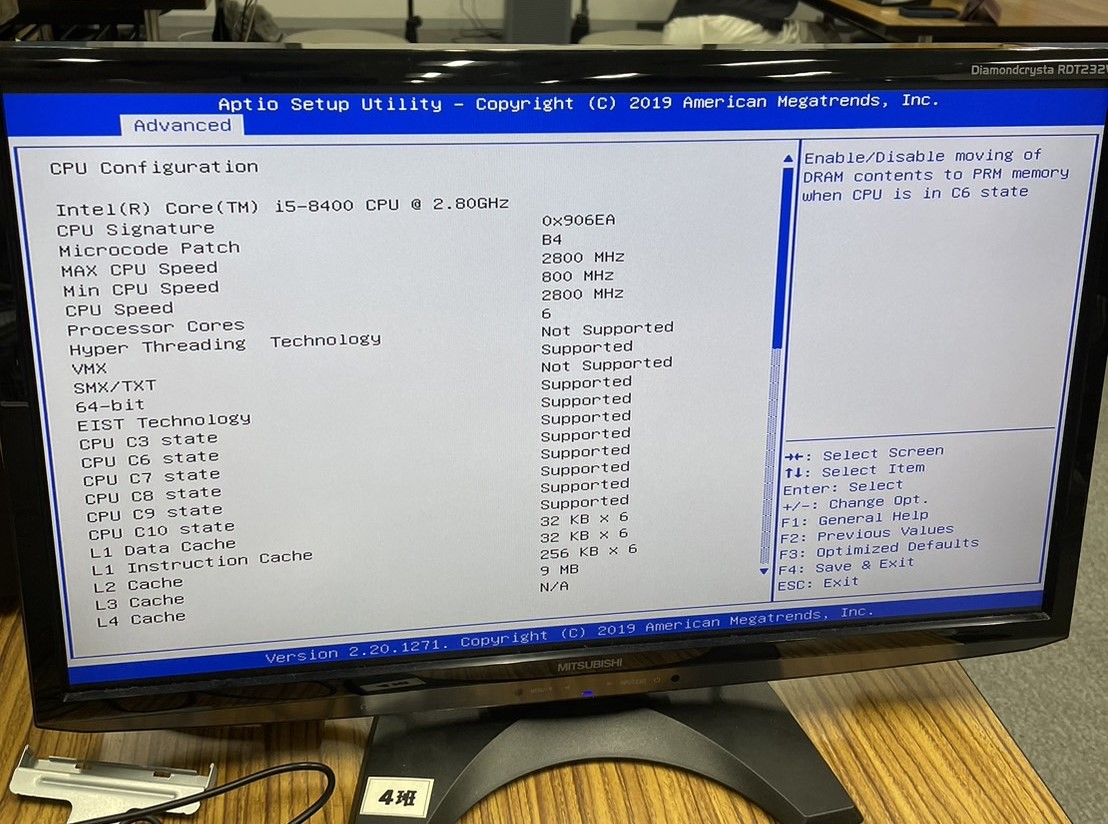
\includegraphics[width=0.5\textwidth]{bios1.jpg} % 画像を挿入、幅をページ幅に合わせる
  \caption{BIOSでCPU名の確認} % キャプションを追加
  \label{fig:bios1} % ラベルを追加
\end{figure}

\subsubsection{BIOSの設定}

BIOSのboot画面から, Dual Boot Order 1にCD, DVDが来るように設定した.
この時の状況を図\ref{fig:bios2}に示す.
change and saveを選択した.

\begin{figure}[H] % 画像を挿入する環境を開始
  \centering
  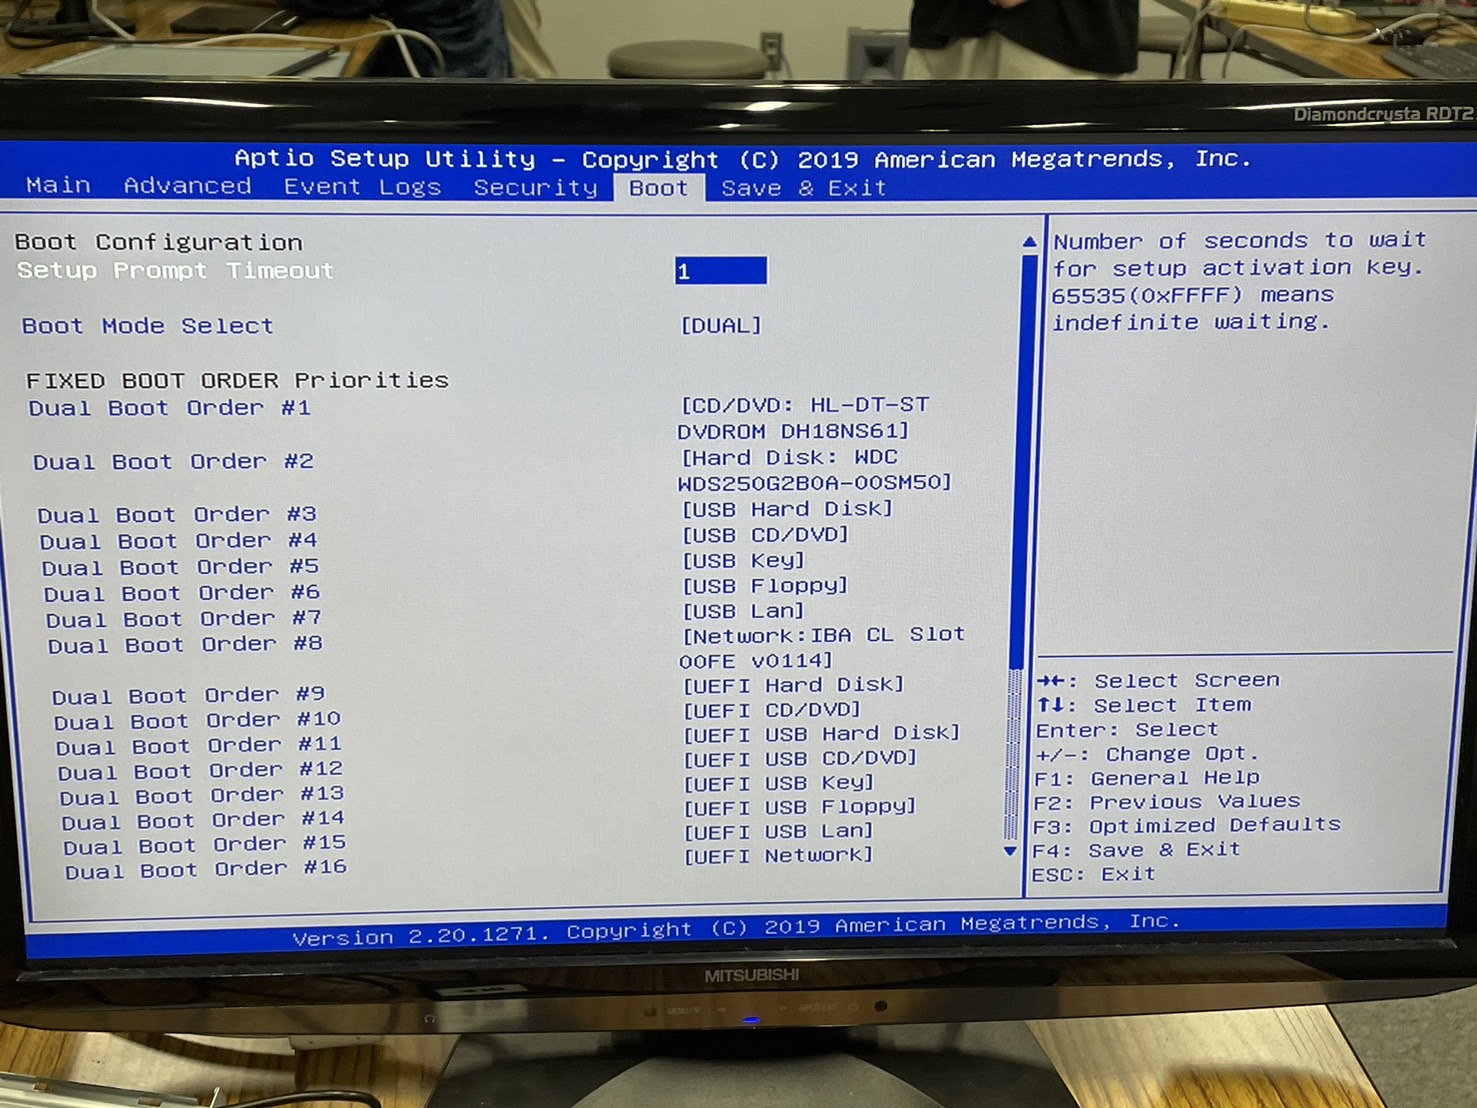
\includegraphics[width=0.5\textwidth]{bios2.jpg} % 画像を挿入、幅をページ幅に合わせる
  \caption{BIOSの設定} % キャプションを追加
  \label{fig:bios2} % ラベルを追加
\end{figure}

\subsubsection{Linux のインストール}

Ubuntu 20.04 LTS インストール用のCD/DVD-ROMを光学ドライブに⼊れてPCを再起動させた.
Ubuntuをインストールを選択し, Keyboard layoutをJapanese, Japaneseに選択した.
Normal installation, Erase disk and install Ubuntsu, continue, Japan Timeを選択した.
Your name をcs-4, Your computer's name をcs4-Super-Server, Pick a usernameを cs-4にした.
Choose a password とconfirm your password に適切なパスワードを設定した.
その後, Restart Nowを選択し, 再起動した. 

コマンドプロンプトから, sudo chmod 666 /dev/ttyS0 コマンドで, アクセス権限を変更した.
パスワードが求められたので, 入力した.

\subsubsection{ネットワークの設定の確認}

まず, /sbin/ip コマンドでip コマンドの構文や利用できるオプション・サブコマンドを確認した.
次に, man ipコマンドで, ip命令のマニュアルを確認した.
そして, ip addr > hoge.txt命令で, ip addr命令の内容をhoge.txtに保存した.
詳細は, 結果や考察で記す.

\subsubsection{SSDにインストールされたOSの消去}

sudo dd if=/dev/zero of=/dev/sda 命令を実行し, OSをアンインストールした.
3分くらい経過した時点でctrl-Cで処理を中断し, シャットダウンした.
再起動し, OSが消去されたことを確認した.


\subsection{実験結果}

\subsubsection{ネットワークの設定の確認}

/sbin/ip コマンドで出力された内容を図\ref{fig:sbin}に示す. 
ip  OPTIONS  OBJECT  COMMAND | helpというのが, 基本構文であることが分かる.
使用可能な OBJECT(オブジェクト)
link: ネットワークインターフェースに関連するコマンド, 
address: IPアドレスに関連するコマンド, 
route: ルーティングテーブルに関連するコマンド, 
他にはrule, neigh, ntable, tunnel などもある. 

オプションには, 
-f: force(強制)オプション, 
-s: statistics(統計)情報を表示, 
-details: 詳細情報を表示, 
-4, -6: IPv4やIPv6のアドレスのみを表示,
-brief: 概要のみを表示するオプションなどがある. 

man ipコマンドで出力された内容を図\ref{fig:man}に示す. 
NAMEセクション, SYNOPSISセクション, オプションがあることが分かる.
オプションには, -V: バージョンを表示して終了。
-h: 出力を人間が読みやすい形式で表示(human-readable), 
-s: 統計情報を表示, 
-d: 詳細情報を表示, 
-4, -6: IPv4 または IPv6 に限定した情報を表示するなどのものがある.

ip addr > hoge.txt命令で作成されたhoge.txtの内容を図\ref{fig:hoge}に示す. 

1. loはループバックインタフェースを表しており, システム自体にネットワークの接続を行うための仮想インタフェースである. 
LOOPBACK,UP,LOWER UP:インタフェースの状態を示す. LOOPBACKはループバックインタフェースであることを示し, UP はインタフェースが有効であることを表す.
mtu 65536:MTU(最大転送単位)は, インタフェースで転送できる最大パケットサイズ(バイト単位)である. ループバックインタフェースの場合は 65536である.
qdisc noqueue:このインタフェースはキューを持っていないことを示す。ループバックインタフェースには通常、パケットキューは不要である.
inet 127.0.0.1/8:IPv4アドレスで, ループバックアドレス 127.0.0.1 が割り当てられていることを示す. 
/8 はサブネットマスクの範囲を示し, この範囲内のアドレスはループバックとして使われていることを示す.
inet6 ::1/128:IPv6アドレスとして ::1 が割り当てられていることを示す. /128 はその特定のホストを示すIPv6アドレスの範囲である.

2. eno2は有線ネットワークインタフェースを表している.
BROADCAST,MULTICAST,UP,LOWER UP: BROADCASTはブロードキャストがサポートされていること、MULTICASTはマルチキャストがサポートされていることを示す.
mtu 1500: MTUは1500バイトである.
qdisc mq: キューイングディシプリン(qdisc)としてmqが設定されている.
state UP: インタフェースが動作中であることを示している.
link/ether ac:1f:6b:ad:ee:bd: MACアドレス(物理アドレス)は ac:1f:6b:ad:ee:bd であることが分かる.
altname enp2s0: eno2の別名(alternative name)が enp2s0 であることが分かる.
inet 10.10.102.191/16:IPv4アドレスは 10.10.102.191 で, サブネットマスク /16 は 255.255.0.0 である. 
valid lft 21274sec と preferred lft 21274sec: このIPアドレスの有効期間(リース時間)を秒数で示している.
inet6 fe80::d351:2520:fe25:8279/64: リンクローカルIPv6アドレスである. fe80::/64 はリンクローカル範囲を表してる.

3. eno1は別の有線ネットワークインタフェースである.

NO-CARRIER: インタフェースは有効(UP)だが, 物理的にネットワークケーブルが接続されていないことを意味している.
BROADCAST,MULTICAST,UP: ブロードキャストとマルチキャストがサポートされており, インタフェースは有効であることを示す.
state DOWN: インタフェースは物理的に接続されていないため, 動作していない状態であることが分かる.
link/ether ac:1f:6b:ad:ee:bc: MACアドレスは ac:1f:6b:ad:ee:bc である.
altname enp0s31f6: 別名(altname)は enp0s31f6 であることが分かる.

ここからわかることは, 考察に記す.

\begin{figure}[H] % 画像を挿入する環境を開始
  \centering
  \begin{minipage}{0.45\textwidth} % 1つ目の画像の幅をページの45%に設定
    \centering
    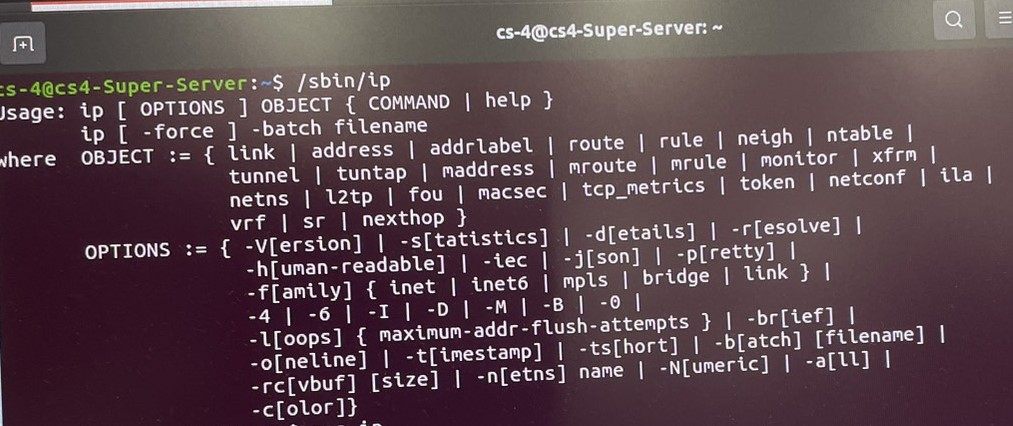
\includegraphics[width=\textwidth]{sbin.jpg} % 画像を挿入、幅をminipage幅に合わせる
    \caption{/sbin/ip コマンド} % キャプションを追加
    \label{fig:sbin} % ラベルを追加
  \end{minipage}
  \hfill % 画像の間にスペースを追加
  \begin{minipage}{0.45\textwidth} % 2つ目の画像の幅をページの45%に設定
    \centering
    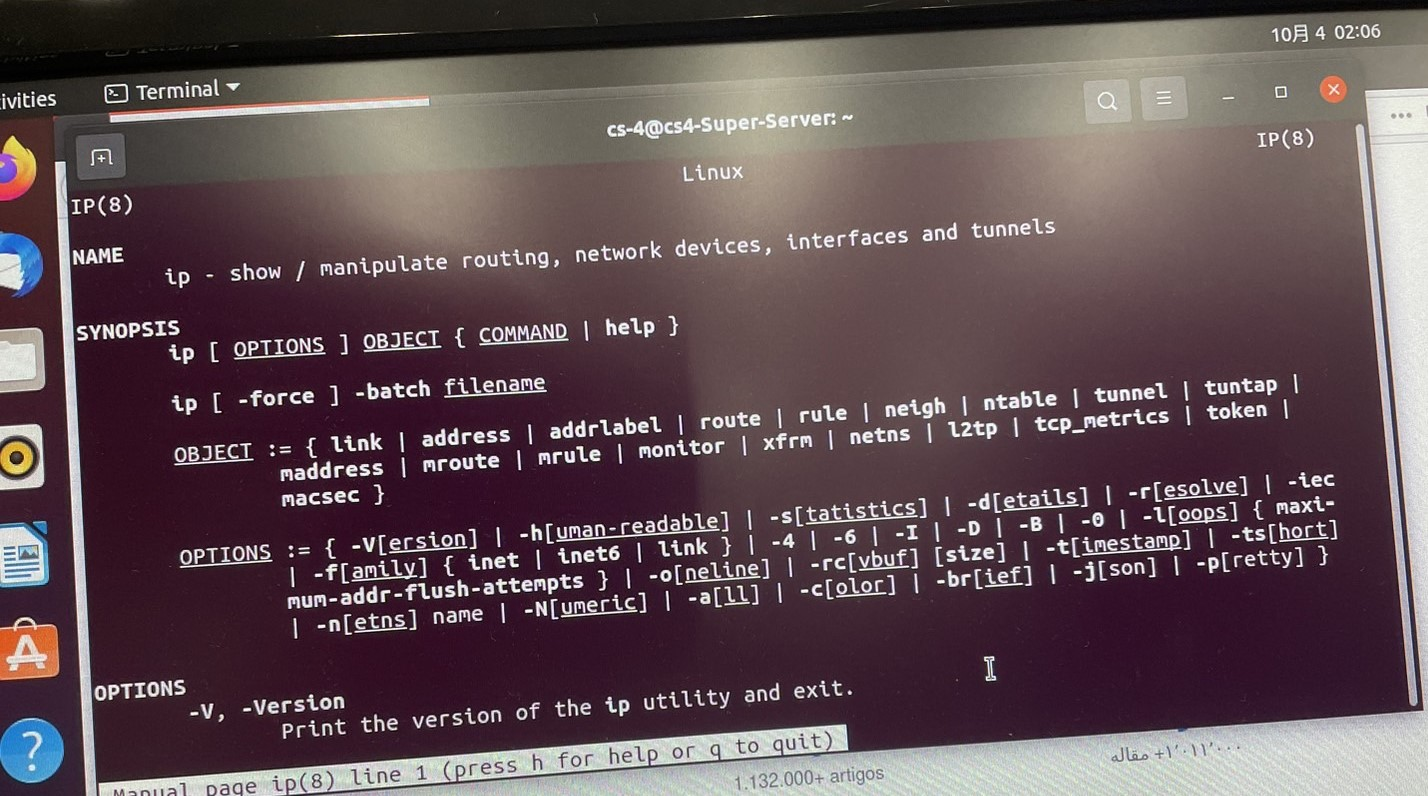
\includegraphics[width=\textwidth]{man.jpg} % 2つ目の画像を挿入
    \caption{man ipコマンド} % キャプションを追加
    \label{fig:man} % ラベルを追加
  \end{minipage}
\end{figure}


\begin{mdframed}
  \begin{verbatim}
    1: lo: <LOOPBACK,UP,LOWER_UP> mtu 65536 qdisc noqueue state UNKNOWN group default qlen 1000
    link/loopback 00:00:00:00:00:00 brd 00:00:00:00:00:00
    inet 127.0.0.1/8 scope host lo
       valid_lft forever preferred_lft forever
    inet6 ::1/128 scope host 
       valid_lft forever preferred_lft forever
    2: eno2: <BROADCAST,MULTICAST,UP,LOWER_UP> mtu 1500 qdisc mq state UP group default qlen 1000
    link/ether ac:1f:6b:ad:ee:bd brd ff:ff:ff:ff:ff:ff
    altname enp2s0
    inet 10.10.102.191/16 brd 10.10.255.255 scope global dynamic noprefixroute eno2
       valid_lft 21274sec preferred_lft 21274sec
    inet6 fe80::d351:2520:fe25:8279/64 scope link noprefixroute 
       valid_lft forever preferred_lft forever
    3: eno1: <NO-CARRIER,BROADCAST,MULTICAST,UP> mtu 1500 qdisc fq_codel state DOWN group default qlen 1000
    link/ether ac:1f:6b:ad:ee:bc brd ff:ff:ff:ff:ff:ff
    altname enp0s31f6	
  \end{verbatim}
  \end{mdframed}
  \begin{figure}[H]
  \caption{hoge.txt}
  \label{fig:hoge}
  \end{figure}


\subsection{考察}

\subsubsection{ネットワークの設定の確認}

図\ref{fig:hoge}のip addr命令のeno2の結果から, ネットワークに接続されているが, IPv4アドレスが 10.10.102.191 であるため, 
これはプライベートネットワークのアドレス空間であると考えられる. このため, インターネットに直接アクセスするためには, 
NAT(ネットワークアドレス変換)が必要である. また, 状態は UP であるため, 正常に動作していると判断できる. 
実際にfirefoxでインターネットに接続したところ, うまくつながった. 


\section{調査課題1-1 最新のPC事情について}

\subsection{メモリ}

まず, DDR, SDRAMのメモリ間の違いについて調べた.

\vspace{0.5cm}

SDRAMの第1世代はDDR SDRAMである. 
これは, サイクルごとに1回受け入れられる同じコマンドを使用されるが, クロックサイクルごとに2つのデータワードを読み書きする.
DDRインターフェイスは, クロック信号の立ち上がりエッジと立ち下がりエッジでデータを読み書きすることでこれを実現できるようになった.

\vspace{0.5cm}

DDR2 SDRAMは読み書きの最小単位が再び2倍になり, 連続する4ワードに達する.
また, バスプロトコルも簡素化され, より高いパフォーマンスを達成した. 特に,「バースト終了」コマンドは削除された。
その結果, 内部RAM動作のクロックレートを上げることなく, SDRAMのバスレートを2倍にできるようになった.

\vspace{0.5cm}

DDR3 SDRAMでは, 最小読み出し/書き込み単位を8連続ワードに倍増させることができるようになった. 
その結果, 内部動作のクロックレートを変更することなく, 幅だけを変更し帯域幅と外部バスレートを再び2倍にできるようになった. 
ただし, 800-1600M転送/秒を維持するために, 内部RAMアレイは100-200Mフェッチ/秒を実行する必要がある.

\vspace{0.5cm}

DDR4 SDRAMは内部プリフェッチ幅を再び2倍にすることはないが, DDR3と同じ8nプリフェッチを使用する. 
(Saki, 2023)

\vspace{0.5cm}

次に, ECCメモリについて, 調べた. ECCメモリは, データのエラーを検出し修正する機能を持つメモリである. 
主にサーバーやクリティカルなシステムで使用され, データの整合性を保つために重要である. 
ECCは, データが破損した際に自動的に修正を行うため, 安定した動作が求められる環境で重宝される. 
また, ECCとは, データを伝送・記録する際に発⽣する誤りを受信や読み出しの際に検出し, 
訂正することができるように付加される符号である. (e-Words, 2024)


\vspace{0.5cm}

次に, CASレイテンシ(Column Address Strobe latency)について調べた. 
CASレイテンシは, アクセスしたい記憶素子の列アドレスを指定する信号を送出してからデータが届き始めるまでにかかる遅延時間のことである.
これは, コンピュータのメインメモリに用いられるDRAM(Dynamic RAM)の特性および性能指標の一つである.  
この値が小さいほど高速に入出力できる. 

CASレイテンシはクロック信号何回分に相当するかで表される. 
CL=2のときはCASレイテンシが2クロック分必要であることを示している. 
(e-Words, 2024)

\vspace{0.5cm}

最後に, デュアルチャンネルメモリについて調べた. 
デュアルチャンネルメモリは, 2つのメモリモジュールをペアで使用する技術である. これにより, データの帯域幅が倍増し, 
システム全体のパフォーマンスが向上する. デュアルチャンネルモードでは, メモリが同時にデータを読み書きできるため, 
アプリケーションの応答性や処理速度が改善される.(crucial, 2024)


\subsection{ビデオカード}

ビデオカードとは, コンピュータの映像を信号として, 出力または入力する機能を拡張カードとして独立させたものである.
「ビデオボード」「グラフィックカード」「グラフィックボード(俗称グラボ)」「グラフィックスカード」
「グラフィックスボード」「グラフィックスアクセラレーターカード」ともいう. 

\vspace{0.5cm}

ゲームや3Dグラフィックスなど, ビデオカードはゲーム用途で広く使用されてきた. 
特に, NVIDIA RTX 4090 や AMD Radeon RX 7900 XT などの高性能ビデオカードは, 
最新のゲームでレイトレーシングや高度なグラフィック処理を実現している. 
これらのカードは, 特にグラフィックのリアルさやフレームレートを向上させるため, ゲーマーにとって必須のツールとなっている.

\vspace{0.5cm}

最近では、GPUは人工知能(AI)や機械学習にも大きな役割を果たしている. 
例えば, ディープラーニングのトレーニングや推論処理に広く採用されている. 
ビデオカードは大規模なデータセットを処理するための並列処理能力に優れており, 特にAI開発において高いパフォーマンスを発揮する.

\vspace{0.5cm}

ビデオカードの最新の動向として, 現在と10年前のビデオカードの性能を調査する. 代表的なビデオカードとして, NVIDIA GeForceの製品で比較する.
最新の製品をGeForce RTX 4090, 10年前の製品をGeForce GTX 780とする. 
それぞれ, 図\ref{fig:4090}, 図\ref{fig:780}に示す.

\vspace{0.5cm}

比較項目として, メモリサイズ, コアクロック周波数, 最大消費電力450 W, G3D Markの値を用いる.

メモリサイズは, グラフィックス処理に必要なデータ(テクスチャ、シェーダ、フレームバッファなど)を一時的に保存する.
特に高解像度のグラフィックや3Dレンダリングを扱う場合に, このメモリが重要な役割を果たす.

コアクロック周波数は, ビデオカードのコアが1秒間に処理できる命令のサイクル数を示す.

最大消費電力は, ビデオカードが最大パフォーマンスを発揮する際の電力消費量を意味する.

G3D Mark はPassMark Softwareが提供しているベンチマークテストの結果として算出され, 
GPUのグラフィック処理能力を測るために広く利用されている.

\begin{table}[H] % ここで[h]は表の位置をこの場所にすることを指定します
  \centering % 表を中央に配置
  \caption{ビデオボードの性能比較}
  \begin{tabular}{|c|c|c|c|c|} 
  \hline % 上の横線
  ビデオボード名 & メモリサイズ & コアクロック周波数 & 最大消費電力 & G3D Mark\\ \hline % 行の内容と行間の横線
  GeForce RTX 4090 & 24576 MB & 2230 MHz & 450 W & 38569 \\ \hline
  GeForce GTX 780 & 6144 MB & 863 MHz & 250 W & 8003 \\ \hline

  \end{tabular}
  \label{tab:gpu} % 表を参照するためのラベル
\end{table}

表\ref{tab:gpu}にあるように
GeForce RTX 4090の性能について, メモリサイズは24576 MB, コアクロック周波数 2230 MHz, 最大消費電力450 W, 
PassMark Software提供しているベンチマークテストG3D Markの結果は38569である.

GeForce GTX 780の性能について, メモリサイズは6144 MB, コアクロック周波数 863 MHz, 最大消費電力250 W, 
G3D Markの結果は8003である. (PassMark, 2024)

メモリーサイズは約4倍, コアクロック周波数は約3倍, G3D Markの結果は約5倍と大幅に性能が良くなっていることがわかる.
それに対し, 最大消費電力は約2倍しか大きなっておらず, 電力効率は良くなっているといえる.

\begin{figure}[H] % 画像を挿入する環境を開始
  \centering
  \begin{minipage}{0.45\textwidth} % 1つ目の画像の幅をページの45%に設定
    \centering
    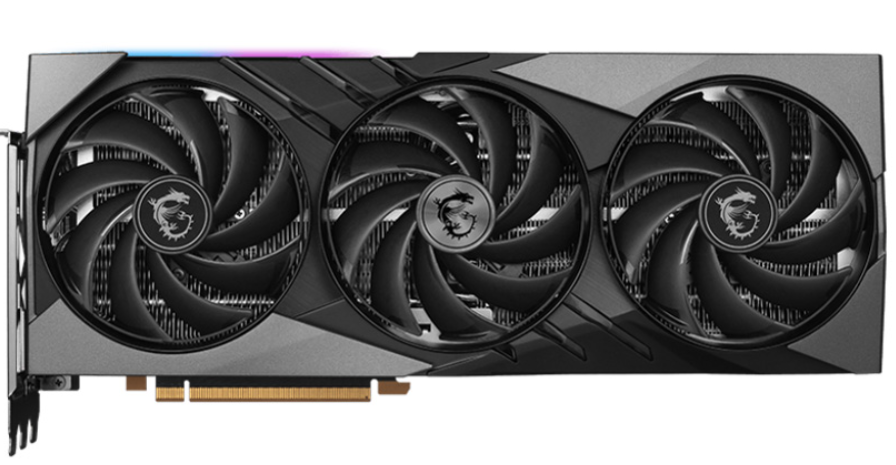
\includegraphics[width=\textwidth]{4090.png} % 画像を挿入、幅をminipage幅に合わせる
    \caption{GeForce RTX 4090} % キャプションを追加
    \label{fig:4090} % ラベルを追加
  \end{minipage}
  \hfill % 画像の間にスペースを追加
  \begin{minipage}{0.45\textwidth} % 2つ目の画像の幅をページの45%に設定
    \centering
    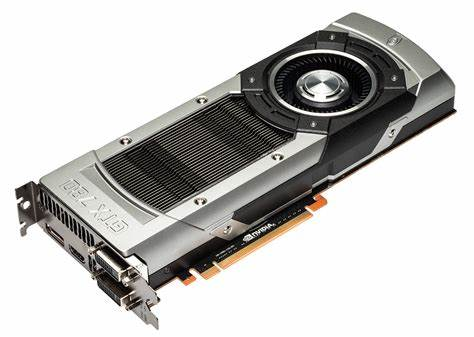
\includegraphics[width=\textwidth]{780.jpg} % 2つ目の画像を挿入
    \caption{GeForce GTX 780} % キャプションを追加
    \label{fig:780} % ラベルを追加
  \end{minipage}
\end{figure}

\section{まとめ}

\subsection{実験を通して分かったこと}
PCパーツの役割や組み立て方についての知識を得ることができた.

\subsection{工夫したこと}
実験で行ったことについて逐一メモを取り, 後から確認しやすいようにした.

\subsection{反省点}
Linuxをインストールする際のユーザ名やパスワードの設定で, 仕様書をよく読まずに
間違ったものを設定してしまった. 今回は一日限りの実験で, 使用後にアンインストールしたので大きな問題にはならなかったが, 
他の実験ではこのようなことが起きないように注意したい. 

\begin{thebibliography}{99} % 最大ラベル幅を99に設定
  
  \bibitem{lamport1994latex}
  Saki: 
  \emph{SDRAMとは DDR2、DDR3、DDR4メモリの違い}. \\
  https://jp.minitool.com/lib/sdram.html  2023.

  \bibitem{lamport1994latex}
  e-wWrds: 
  \emph{誤り訂正符号 【ECC】}. \\
  \verb|https://e-words.jp/w/%E8%AA%A4%E3%82%8A%E8%A8%82%E6%AD%A3%E7%AC%A6%E5%8F%B7.html|  2023.

  \bibitem{lamport1994latex}
  e-wWrds: 
  \emph{CASレイテンシ}. \\
  \verb|https://e-words.jp/w/CAS%E3%83%AC%E3%82%A4%E3%83%86%E3%83%B3%E3%82%B7.html|  2024.

  \bibitem{lamport1994latex}
  crucial: 
  \emph{デュアルチャネルメモリとは?}. \\
  \verb|https://www.crucial.jp/articles/about-memory/what-is-dual-channel-memory|  2024.

  \bibitem{lamport1994latex}
  PassMark: 
  \emph{High End Video Card Chart}. \\
  https://www.videocardbenchmark.net/high\verb|_end_|gpus.html  2024.

\end{thebibliography}


\end{document}